% Fig 5: QNN as truncated Fourier series. Green = trainable blocks -> Fourier
% coefficients; orange = data-encoding blocks -> frequency spectrum. Formula
% colors are saturated so the correspondence is visible (Pavel's comment).
% Drawn at natural size (no resizebox) so all text matches the body font.
\begingroup
% Palette from Fig 8: green = trainable, orange = encoding, violet = readout
\definecolor{trainFill}{RGB}{38,200,110}
\definecolor{encFill}{RGB}{255,167,51}
\definecolor{readFill}{RGB}{99,110,200}
\tikzset{
  qwire/.style={line width=0.7pt},
  tgate/.style={draw=trainFill!60!black, line width=0.8pt, rounded corners=2pt, fill=trainFill,
                minimum width=1.05cm, minimum height=0.6cm, inner sep=2pt},
  egate/.style={draw=encFill!60!black, line width=0.8pt, rounded corners=2pt, fill=encFill,
                minimum width=1.15cm, minimum height=0.6cm, inner sep=2pt},
}
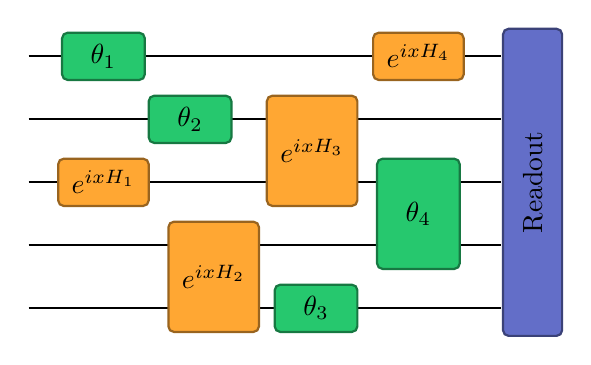
\begin{tikzpicture}[x=1cm,y=1cm]
% wires
\foreach \y in {0,-0.8,-1.6,-2.4,-3.2}{
  \draw[qwire] (0,\y) -- (6.0,\y);
}
% trainable (green) blocks
\node[tgate] at (0.95, 0)    {$\theta_1$};
\node[tgate] at (2.05,-0.8)  {$\theta_2$};
\node[tgate] at (3.65,-3.2)  {$\theta_3$};
\node[tgate, minimum height=1.4cm] at (4.95,-2.0) {$\theta_4$};
% encoding (orange) blocks
\node[egate] at (0.95,-1.6)  {$e^{ixH_1}$};
\node[egate, minimum height=1.4cm] at (2.35,-2.8) {$e^{ixH_2}$};
\node[egate, minimum height=1.4cm] at (3.6,-1.2) {$e^{ixH_3}$};
\node[egate] at (4.95, 0)    {$e^{ixH_4}$};
% readout
\node[draw=readFill!60!black, line width=0.8pt, rounded corners=2pt, fill=readFill,
      minimum width=3.9cm, minimum height=0.75cm, rotate=90, font=\rmfamily]
      at (6.4,-1.6) {Readout};
\end{tikzpicture}%
\endgroup
